\section{LED Driver}
The brick sorter relies on the varying reflective properties of different colors. Using a variety of different color LEDs will enable the sorter to detect different color bricks. This section will describe in detail the decisions made in designing the circuit used for the LEDs and the photo diode as well as presenting the code responsible for driving the LEDs. 

\subsection{Circuit Design}
\begin{figure}[h!]
	\begin{center}
		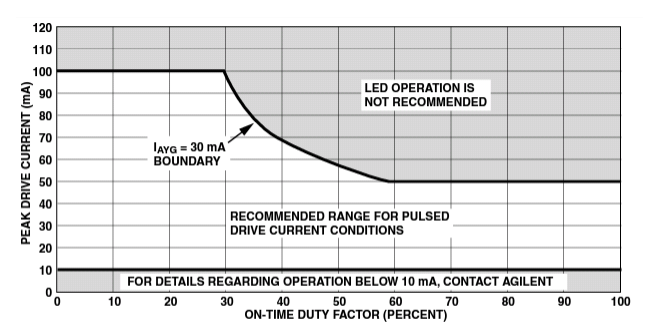
\includegraphics[width=\linewidth]{images/overdrive}
	\end{center}
	\caption{The white region denotes the area in which the LED can safely be driven.}
	\label{fig:overdrive}
\end{figure}
The switching of the LEDs is done using bipolar junction transistors (BJTs). The BJTs are wired as a simple switching circuit as in figure \ref{circ:ledswitch}. $V_{\text{c}}$, the switching signal, will be generated using an FPGA.
In order to achieve the highest possible light intensity from the LEDs they will be overdriven. Figure \ref{fig:overdrive} is an excerpt from \cite{avago}. This graph shows that the LEDs can be safely driven at 100mA so long as the duty cycle of $V_{\text{c}}$ does not exceed 30\%. Driving the LEDs at 100mA implies that $I_c=100\text{mA}$. 

For a BJT:
\begin{eqnarray}
I_c=&I_b\cdot h_{\text{FE}}\\
I_b=&\frac{V_{\text{c}}-V_{be}}{R_1}
\end{eqnarray}
Looking at the datasheet of the BC547b the dc current gain of this transistor is found to be
\begin{eqnarray}
	h_{\text{FE}}=200 \Rightarrow I_b = 0.5\text{mA}
\end{eqnarray}
Lastly, according to figure \ref{fig:vbe} from the datasheet of the BC547b, when $I_c = 100$mA $V_{be}=0.8$v.
Since the BJT is used as a switch it is desirable that it is driven to saturation quickly to avoid dissipating power in the component. Therefore, $I_b$ is doubled and 
\begin{eqnarray}
	R_1 = \frac{V_{\text{c}}-V_{be}}{I_b\cdot 2} = 2.5\text{k}\Omega
\end{eqnarray}

\begin{figure}[h!]
	\centering
	\begin{subfigure}[b]{.48\linewidth}
		\begin{circuitikz}
			\draw (0,0) 
			node[npn](npn1){}
			(npn1.base) ++(-2,0) node[name=r1left]{}
			to[R=$R_1$,o-,i=$I_b$] ++(2,0) ++(-2,0)node[left]{$V_{\text{c}}$}
			(npn1.base) ++(0.75,0) node[right]{BC547b}
			(npn1.emitter) 
			node[ground](GND){}
			(npn1.collector) ++(0,4) node[name=d_top]{}
			to[D=$LED$,o-]++(0,-2) 
			to[R=$R_2$,i=$I_c$]++(0,-2)
			(d_top) node[above]{$V_{cc}$}
			;\end{circuitikz}
		\caption{Switching circuit for single LED}
		\label{circ:ledswitch}
	\end{subfigure}
	\begin{subfigure}[b]{.48\linewidth}
		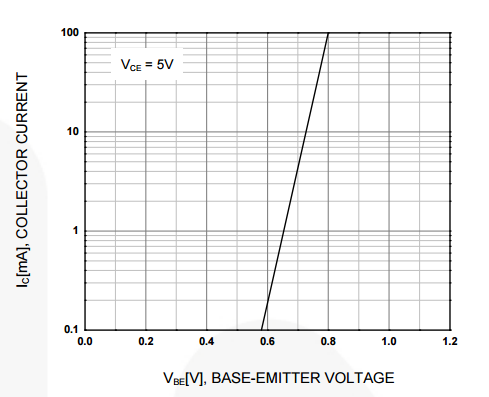
\includegraphics[width=\linewidth]{images/vbe}
		\caption{Graph of $I_c$ as a function of $V_be$.}
		\label{fig:vbe}
	\end{subfigure}
	\caption{(a)LED Circuit, three of these are combined to drive the red, green and blue LEDs used in this application. (b) Graph from the datasheet of the BC547p showing the correlation between collector current and base-emitter voltage.}
\end{figure}
\begin{figure}[h!]
	\begin{center}
		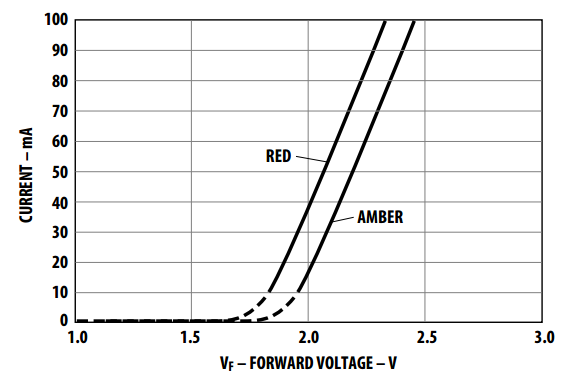
\includegraphics[width=0.75\linewidth]{images/redvd}
	\end{center}
	\caption{Current as a function of forward voltage for the red diode.}
	\label{fig:ledcurrent}
\end{figure}
Finding $R_2$ is done using the datasheets of the LEDs. figure \ref{fig:ledcurrent} shows the correlation between the voltage drop across the diode and the current through the diode.
According to these figures the red LED will have a voltage drop $V_d = 2.3$v and the green and blue LEDs will $V_d = 4$v. This results in 
\begin{eqnarray}
	R_{2\_\text{red}}=& \frac{V_{cc}-V_d}{I_c} &= 97\Omega \\
	R_{2\_\text{green}}=&R_{2\_\text{blue}} = \frac{V_{cc}-V_d}{I_c} &= 80\Omega
\end{eqnarray}

This next part of the circuit is responsible for detecting the reflected light and amplify the signal generated by the photodiode such that it can be processed by the ADC. A diagram of the circuit used can be seen in figure \ref{circ:unfiltered}.
The output voltage of this circuit is determined by:
\begin{eqnarray}
	V_{\text{out}}=&I_{\text{in}}\cdot R_f\\
	R_f =& R_1+R_{\text{pot}}
\end{eqnarray}
When an LED is flashed onto a same-colored brick, the output of the op-amp is expected to be $V_{\text{out}} = V_{\text{sat}}$, the saturation voltage. By experimentation this was found to be $V_{\text{sat}}=3.78$v.

$I_{\text{in}}$ was determined by making the circuit as seen in figure \ref{circ:iinmeasure}. By reflecting the light from the LEDs off of the bricks and onto the photodiode, the maximum current to be expected generated from the photodiode was found to be $I_{\text{in}}=10\mu$A.
This results in $R_f=378\text{k}\Omega$, however, it was found that applying this resistor causes the blue brick to also saturate the op amp when shining the green LED. Additionally, when mounting the LED assembly to the acrylic slide, the slide itself was found to enlarge $I_{\text{in}}$ by a significant margin. Due to these factors $R_f$ was finally dimensioned using a 1M$\Omega$ potentiometer. 

\begin{figure}[h!]
  	\centering
	\begin{subfigure}[b]{.49\linewidth}
		\resizebox{\linewidth}{!}{
			\begin{circuitikz}
				\draw(0,0) 
					node[op amp] (opamp) {}
				(opamp.-) ++(-2,-1) 
					node[ground]{} to[short] ++(0,1)
						to[pD] (opamp.-)
				(opamp.-) to[short] ++(0,1) coordinate(capleft)
					to[R=$R_1$] ++(2,0)
						to[vR=$R_\text{pot}$] ++(2,0) coordinate(pot)
				(opamp.out) -| (pot) coordinate(conn)
					to[short] (pot)
				(opamp.+) to[short] ++(0,-0.5)
					node[ground]{}
			;\end{circuitikz}
		}
		\caption{Unfiltered version.}
		\label{circ:unfiltered}		
	\end{subfigure}
	\begin{subfigure}[b]{.49\linewidth}
		\resizebox{\linewidth}{!}{
			\begin{circuitikz}
				\draw(0,0) 
				node[op amp] (opamp) {}
				(opamp.-) ++(-2,-1) 
				node[ground]{} to[short] ++(0,1)
				to[pD] (opamp.-)
				(opamp.-) to[short] ++(0,1) coordinate(capleft)
				to[R=$R_1$] ++(2,0)
				to[vR=$R_\text{pot}$] ++(2,0) coordinate(pot)
				(opamp.out) to[short] (opamp.out -| pot) coordinate(conn)
				to[short] (pot)
				(opamp.+) to[short] ++(0,-0.5)
				node[ground]{}
				(capleft) to[short] ++(0,1) coordinate(capleftup)
				to[C=$C_f$] (capleftup -| pot)
				to[short] (pot)
				;\end{circuitikz}
		}
		\caption{Filtered version.}
		\label{circ:filtered}
	\end{subfigure}
   	\caption{Photo diode amplifier circuit}
   	\label{circ:photodiode}
\end{figure}

Table \ref{tab:ledtable} shows the various responses of the photodiode when exposed to the different LEDs and bricks.

\begin{table}
	\centering
	\begin{tabular}{| c | c | c | c | c |}
		\hline
		\diagbox{LED}{BRICK}& R & G & B & A\\
		\hline
		R & 2.97 & 1.11 & 1.30 & 1.66\\
		\hline
		G & 1.71 & 3.34 & 2.81 & 2.49\\
		\hline
		B & 1.78 & 2.00 & 3.86 & 2.38\\
		\hline
	\end{tabular}
	\caption[Response from photodiode circuit.]{Response from photodiode circuit. Each color LED; red, green and blue is flashed while each color brick is used as the reflective surface.}
	\label{tab:ledtable}
\end{table}
\subsection{LED Driver}
\subsection{Circuit Testing}
In testing, a significant amount of oscillation appeared on the output of the op amp. See figure \ref{fig:oscillation}. To avoid issues when digitizing the signal with the ADC, it will be filtered by applying a compensation capacitor in parallel with $R_f$, see figure \ref{circ:filtered}.

\begin{figure}[h!]
	\centering
	\begin{subfigure}{\linewidth}
		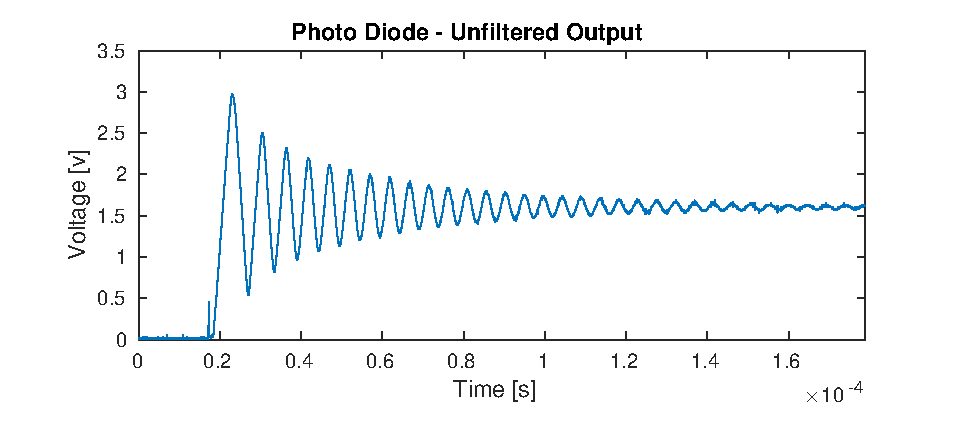
\includegraphics[width=\linewidth]{images/unfiltered}
		\caption{Unfiltered output.}
		\label{fig:oscillation}
	\end{subfigure}\\
	\begin{subfigure}{\linewidth}
		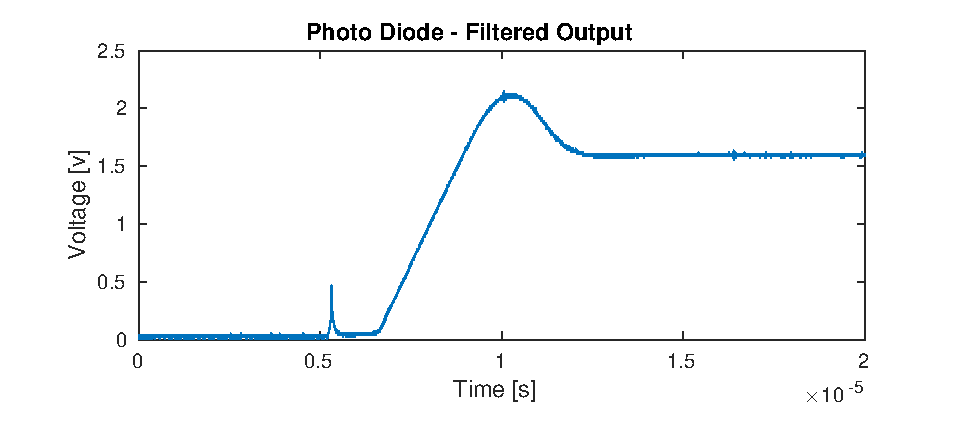
\includegraphics[width=\linewidth]{images/filtered}
		\caption{Filtered output.}
		\label{fig:nooscillation}
	\end{subfigure}
	\caption{Response of the photodiode amplifier circuit.}
	\label{fig:photoresponse}
\end{figure}

 According to \cite{mec} the compensation capacitor is dimensioned using
$$f_c=\frac{1}{2\Pi R C}$$
The oscillation happens at $\approx 138\text{kHz}$ and $R = R_f = 240\text{k}$ this results in 
$$C = 4.8\text{pF}$$
The filtered signal can be seen in figure \ref{fig:nooscillation}. After filtering there is still a significant settling time, $T_{\text{s}}$, before the signal can be safely digitized. $T_{\text{s}}$ varies with the amplitude of the final signal, therefore a conservative time before sampling with the ADC must be set. 
On figure \ref{fig:settletime} it can be seen that the settling time is an expected $T_{\text{s}}=12.65\mu$s.
\begin{figure}[h!]
	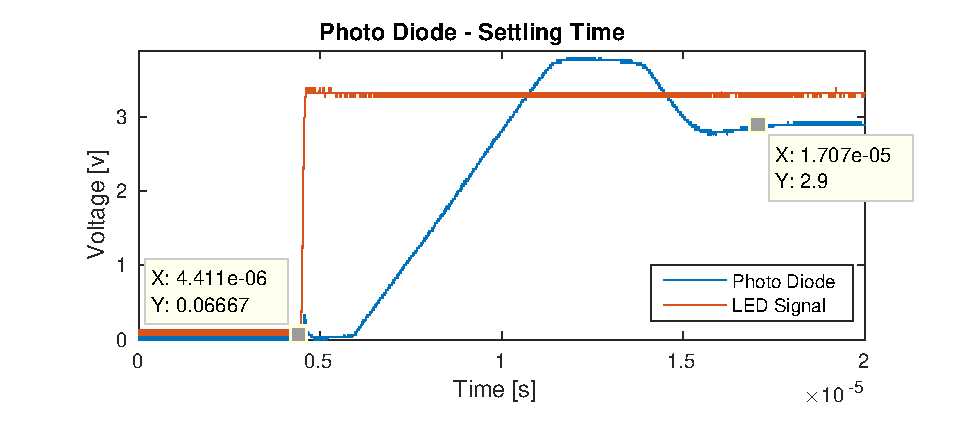
\includegraphics[width=\linewidth]{images/settle}
	\caption{Worst case settling time. When LED signal goes high, the photo diode is expected to have settled after $T_{\text{s}}=12.65\mu$s.}
	\label{fig:settletime}
\end{figure}